%\documentclass[final,hyperref={pdfpagelabels=false}]{beamer}
\documentclass[final]{beamer}
\usepackage{grffile}
%\mode<presentation>{\usetheme{Singapore}}
\mode<presentation>{\usetheme{I6pd2}}
\usepackage[english]{babel}
%\usepackage[latin1]{inputenc}
\usepackage[utf8]{inputenc}
\usepackage{amsmath,amsthm, amssymb, latexsym}
%\usepackage{times}\usefonttheme{professionalfonts}  % obsolete
%\usefonttheme[onlymath]{serif}
\boldmath
\usepackage[orientation=portrait,size=a0,scale=1.4,debug]{beamerposter}
% change list indention level
% \setdefaultleftmargin{3em}{}{}{}{}{}

%\setbeamercolor{structure}{fg=ta3skyblue}

%\usepackage{snapshot} % will write a .dep file with all dependencies, allows for easy bundling

\usepackage{array,booktabs,tabularx}
\newcolumntype{Z}{>{\centering\arraybackslash}X} % centered tabularx columns
\newcommand{\pphantom}{\textcolor{ta3aluminium}} % phantom introduces a vertical space in p formatted table columns??!!

\listfiles

%%%%%%%%%%%%%%%%%%%%%%%%%%%%%%%%%%%%%%%%%%%%%%%%%%%%%%%%%%%%%%%%%%%%%%%%%%%%%%%%%%%%%%
\graphicspath{{figures/}}
 
\title{\huge (2-F-56) Histogram of Gradient Orientations of Signal Plots applied to Brain Computer Interfaces}
\author{Ramele Rodrigo, Santos Juan Miguel, Villar Ana Julia}
\institute[Instituto Tecnológico de Buenos Aires]{Computer Engineering Department,Graduate School of Engineering, Buenos Aires, Argentina}
\date[May. 22nd, 2018]{May. 22nd, 2018}

%%%%%%%%%%%%%%%%%%%%%%%%%%%%%%%%%%%%%%%%%%%%%%%%%%%%%%%%%%%%%%%%%%%%%%%%%%%%%%%%%%%%%%
\newlength{\columnheight}
\setlength{\columnheight}{105cm}


%%%%%%%%%%%%%%%%%%%%%%%%%%%%%%%%%%%%%%%%%%%%%%%%%%%%%%%%%%%%%%%%%%%%%%%%%%%%%%%%%%%%%%
\begin{document}
\begin{frame}

  \begin{columns}
    % ---------------------------------------------------------%
    % Set up a column 
    \begin{column}{.49\textwidth}
      \begin{beamercolorbox}[center,wd=\textwidth]{postercolumn}
        \begin{minipage}[T]{.95\textwidth}  % tweaks the width, makes a new \textwidth
          \parbox[t][\columnheight]{\textwidth}{ % must be some better way to set the the height, width and textwidth simultaneously
            % Since all columns are the same length, it is all nice and tidy.  You have to get the height empirically
            % ---------------------------------------------------------%
            % fill each column with content            
            \begin{block}{Introduction}
              \begin{itemize}
              \item \textbf{Where are the waveforms?}
                \begin{itemize}
                \item Through the last fifteen years, many successful projects have proved the feasibility  to transfer information from the Central Nervous System to a computer, machine or robot.
                \end{itemize}
              \item \textbf{BCIs are even now being considered an important branch of Human Computer Interaction.}
                \begin{itemize}
                \item Games, Neuromarketing, Neuroergonomy, lie detection, biometric security, teleprescence.
                \end{itemize}
              \item Although, this widespread usage, the key aspect of BCI still lies in its support into \textbf{Assitive Technologies}.   
                \begin{itemize}
                \item However,  there are many challenges ahead that need to be tackled: \textit{"we yet have an impractical and inaccessible exotica for very specific user groups"}([5])
                \item We need \textbf{New mental paradigms} and \textbf{to get out of the lab into the real world!}
                \end{itemize}
              \end{itemize}               
            \end{block}
            \vfill
            \begin{block}{Histogram of Gradient Orientations}
                  \begin{itemize}
                  \item Cognition is not strictly located within the physiological borders of the brain.  
                  \item Intelligent behaviour emerges out of the interplay between brain, body and world.  Cognition is predominantly Active and Multisensorial  [1,3]
                  \item Spatial Localization: the Tempo Parietal Junction is involved in processes of self-localization, self-identification and is related to the situatedness of agents in their environments. 
                    \begin{itemize}
                    \item We want to verify that if cognition relies strongly on the interaction with the environment and the agent's sensorial loop, then there must be a noteworthy signal feature strong enough to be detected by non invasive EEG.
                    \item We also hypothesize that this signal could be modulated to effectively transmit volition.
                    \end{itemize}
                  \end{itemize}
                  
					\begin{columns}
					\begin{column}{.30\textwidth}
							\centering
                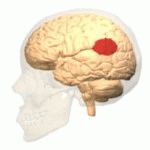
\includegraphics[width=0.80\linewidth]{images/viola/tpj}
					\end{column}
					\begin{column}{.70\textwidth}
							\centering
                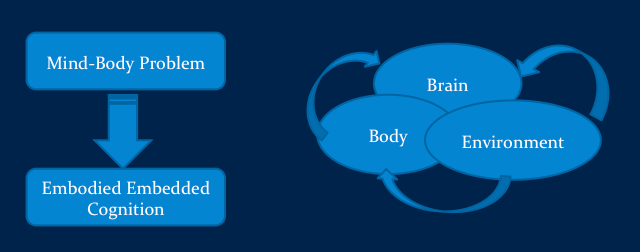
\includegraphics[width=1\linewidth]{images/viola/embodimentsmall}
					\end{column}
					\end{columns}                  
                  
                  
              \vskip-1ex
            \end{block}            
            \vfill
            \begin{block}{Decoding $ \alpha$  waves}
              \begin{itemize}
              \item Alpha (8-13 Hz) waves are an inhibitory signal and are stronger on cognitive idle states when there is an absence of interaction with the environment.
              \item Inside the practical bandwidth of EEG signals ( 0-40 Hz).
              \item Affordable in the terms of Cost, with Wearable Commercial Devices (i.e. EPOC Emotiv).
              \end{itemize}
              
               \begin{columns}
              	\begin{column}{.33\textwidth}
				\centering 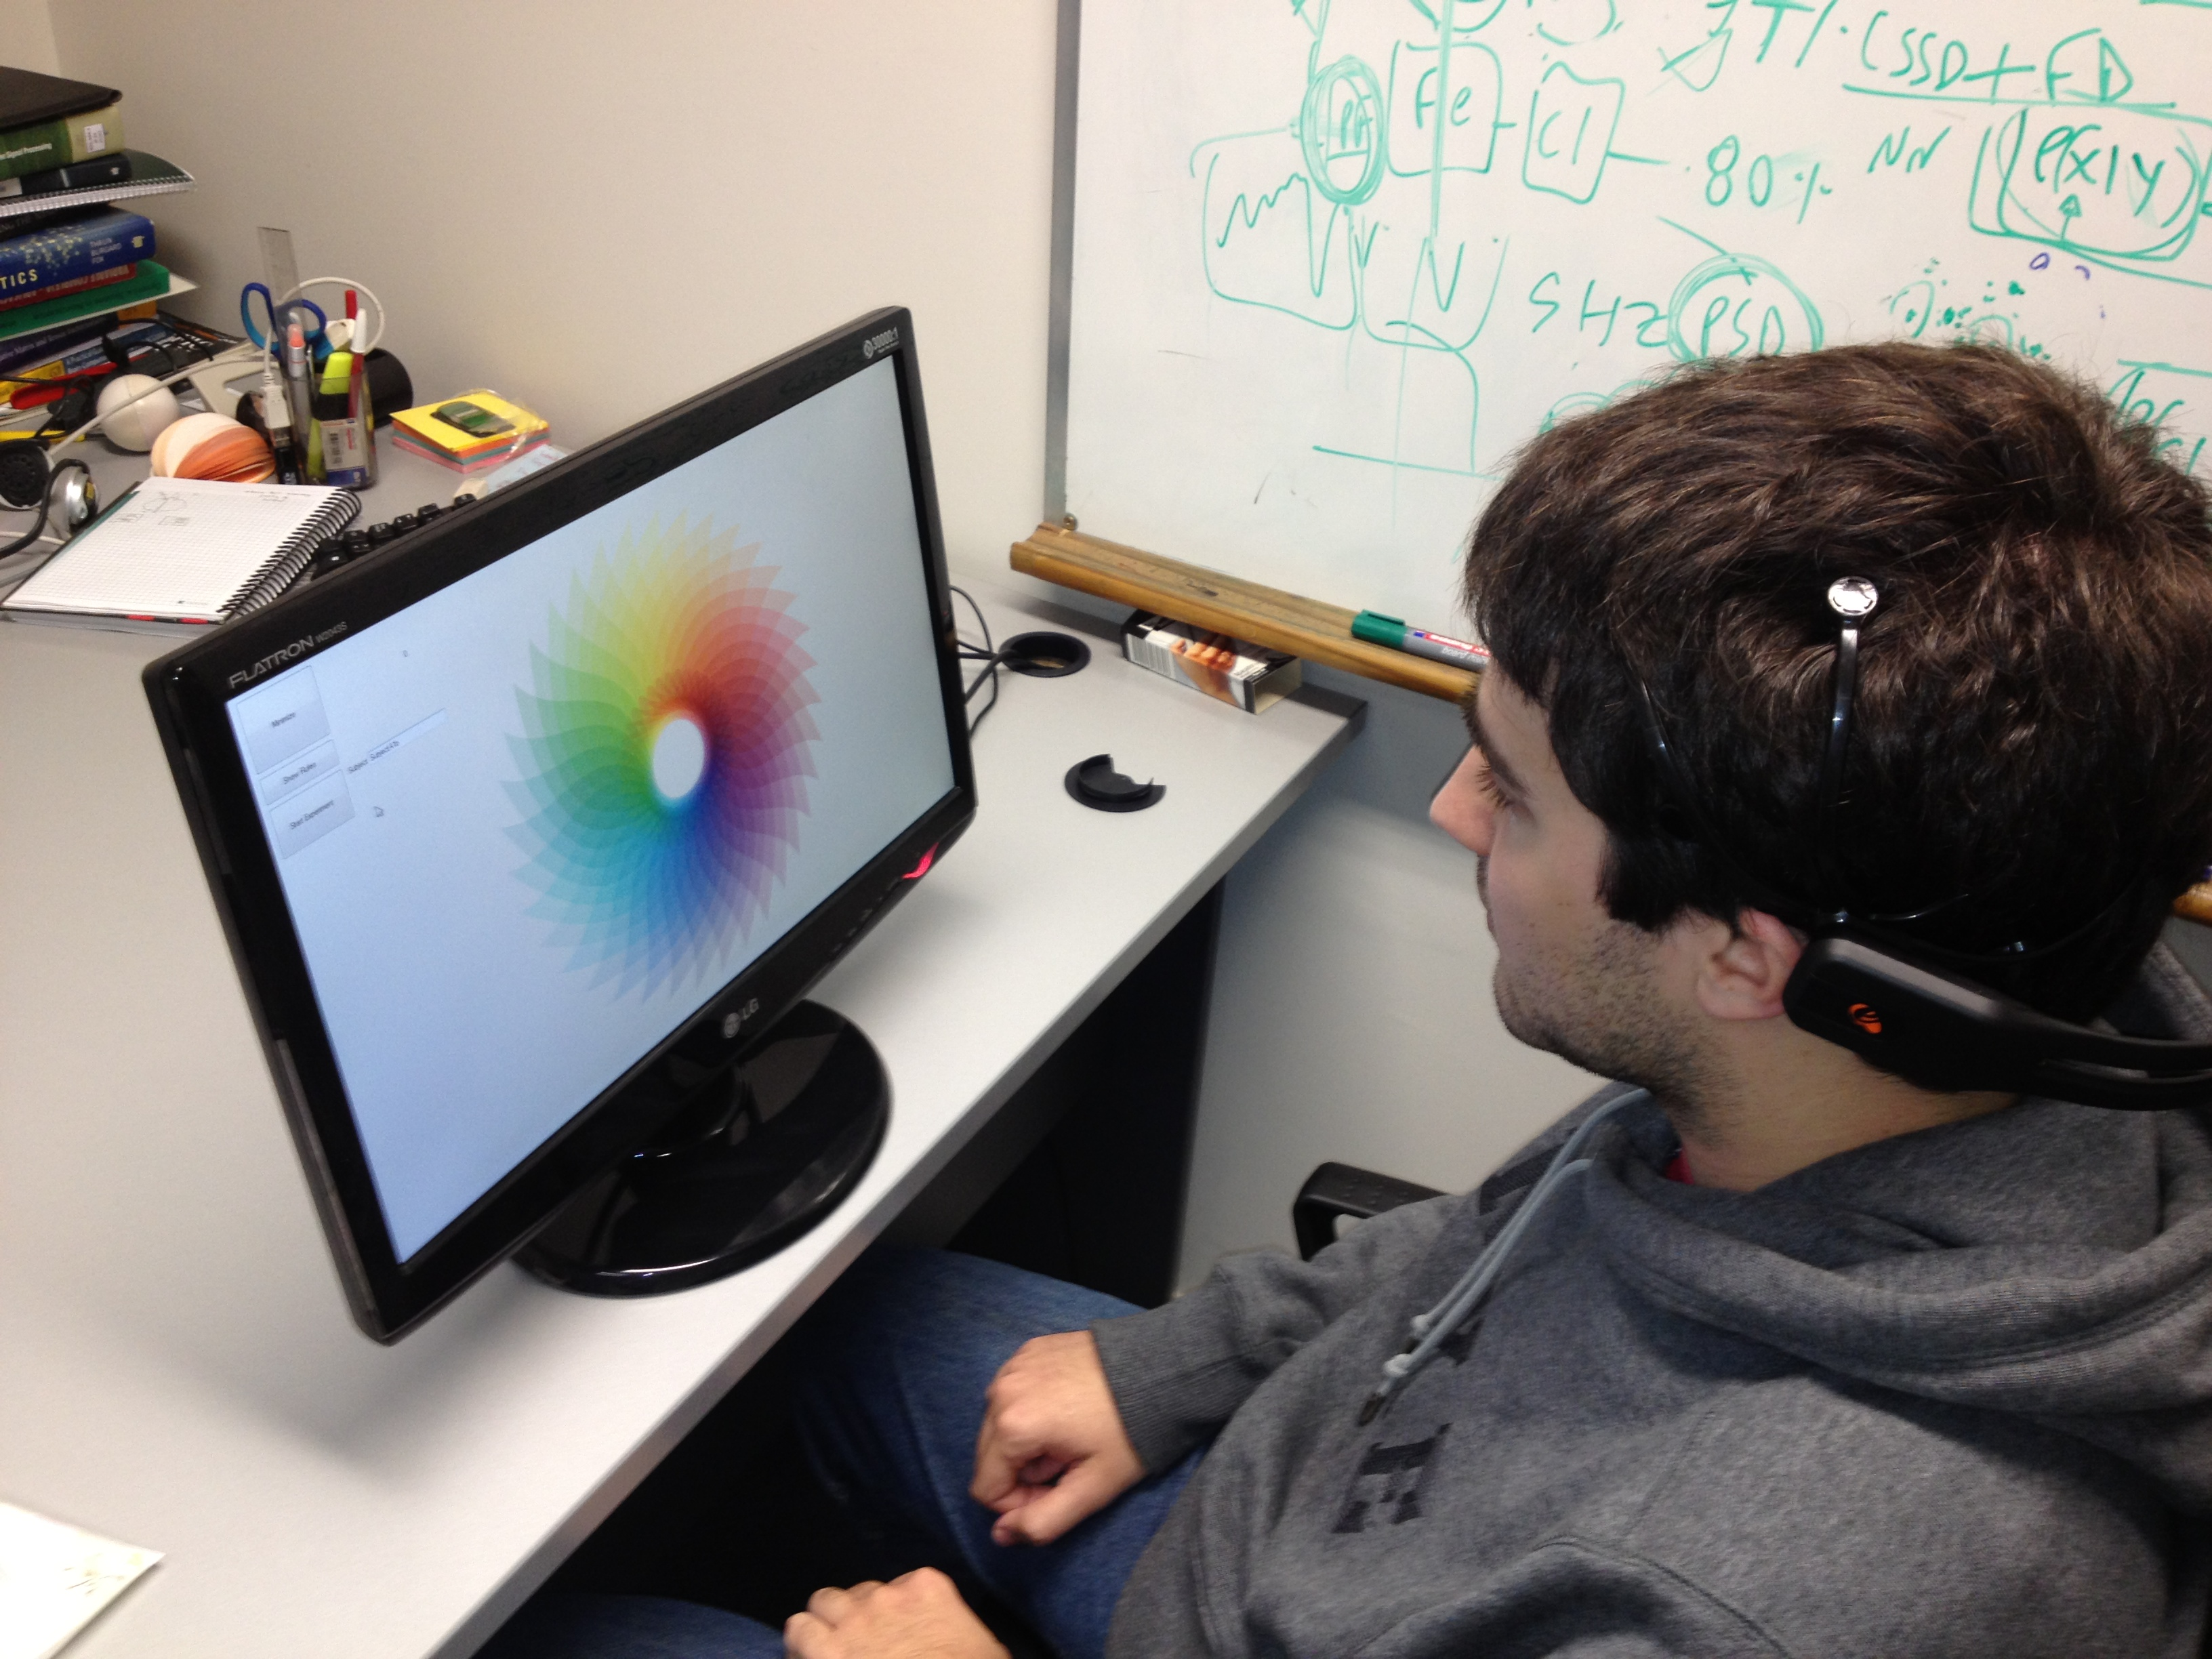
\includegraphics[width=0.95\linewidth]{images/viola/subject}
				\end{column}
				\begin{column}{.33\textwidth}
				\centering 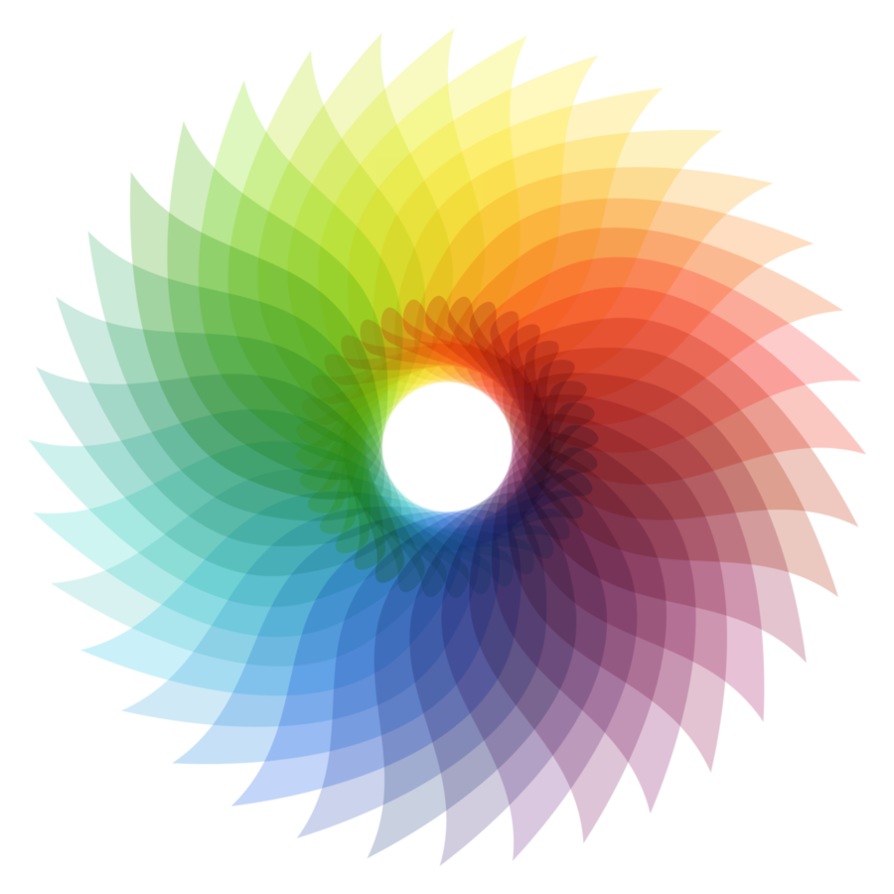
\includegraphics[width=0.95\linewidth]{images/viola/calibration}
				\end{column}
				\begin{column}{.33\textwidth}
				\centering 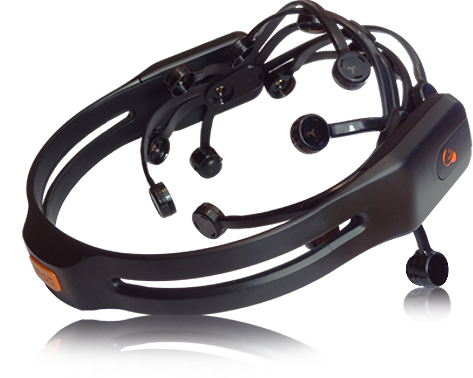
\includegraphics[width=0.95\linewidth]{images/viola/emotivlarge}
				\end{column}
				\end{columns}
				
                \begin{itemize}
                \item \textbf{Protocol}
                \begin{enumerate}
                \item Subject is instructed to count the number of flashes on the sides of an image.  Gazing not allowed ! [4]
                \item Flickering light on both sides of the screen at random frequency rates (similar to Oddball paradigm). 16 trials, $ T =4 s $ each.
                \item 15 healthy voluntary subjects were recruited.
                \end{enumerate}
                
                \item \textbf{Analyze Method}
                \begin{enumerate}
                \item EEGLAB, BCILAB, Matlab, fieltrip
                \item 
                
                \begin{columns}
                \setlength{\tabcolsep}{0em}
              	\begin{column}{.05\textwidth}
				\end{column}
              	\begin{column}{.18\textwidth}
				\centering 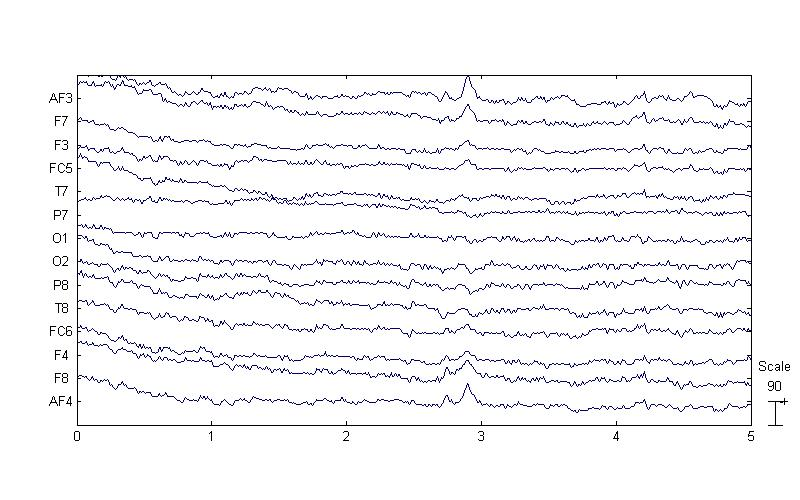
\includegraphics[width=0.95\linewidth]{images/viola/eeglab1}
				\end{column}
				\begin{column}{.18\textwidth}
				\centering 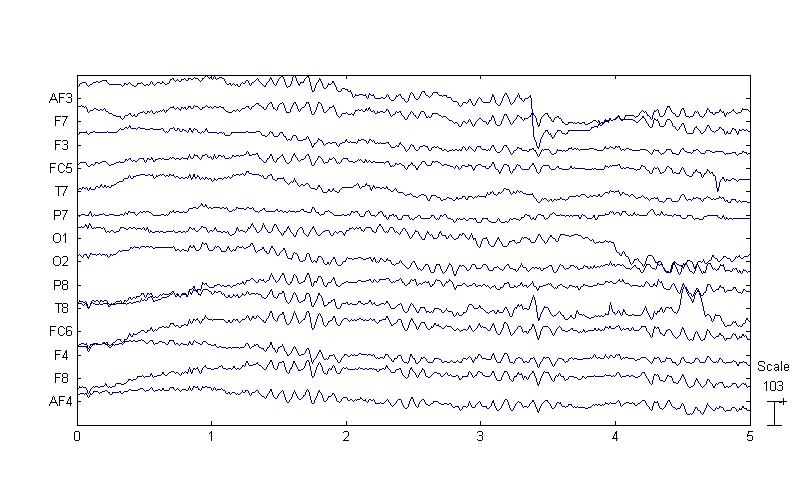
\includegraphics[width=0.95\linewidth]{images/viola/eeglab2}
				\end{column}

				\begin{column}{.78\textwidth}	
				\begin{itemize}
				\item CSP,  band-pass filter to 8-13 Hz.
				\item PSD over each channel
				\item Estimation of winner channel: Left or Right?
				\end{itemize}
                \end{column}  			
				
				\end{columns}
				                
                \end{enumerate}
                
                \item \textbf{Current Results}
                \begin{itemize}
                \item Estimating flickering side: very high error rate: 42 \% !
                \item Is the device accurate ?   Next:  gaze tracker, EOG detection, CSSD.
                \end{itemize}
                \item Work in Progress !!!
                \end{itemize}
            \end{block}
            \vfill
          }
        \end{minipage}
      \end{beamercolorbox}
    \end{column}
    % ---------------------------------------------------------%
    % end the column

    % ---------------------------------------------------------%
    % Set up a column 
    \begin{column}{.49\textwidth}
      \begin{beamercolorbox}[center,wd=\textwidth]{postercolumn}
        \begin{minipage}[T]{.95\textwidth} % tweaks the width, makes a new \textwidth
          \parbox[t][\columnheight]{\textwidth}{ % must be some better way to set the the height, width and textwidth simultaneously
            % Since all columns are the same length, it is all nice and tidy.  You have to get the height empirically
            % ---------------------------------------------------------%
            % fill each column with content
            
            \begin{block}{Electroencephalography}
              \begin{columns}
                \begin{column}{.6\textwidth}
                  \begin{itemize}
                  \item Aging Societies
                    \begin{itemize}
		    \item Estimated for 2025, 800 millions people will be over 65 old.
                    \item 2/3 of them on ''developing'' countries.
                    \item Increased tendency to develop diseases that affect motor pathways.
                    \end{itemize}
                  \item Through technology, provide a better quality of life for more people.
                    \begin{itemize}
                    \item Specially for those affected by diseases or disabilities.
                    \end{itemize}
                  \item Active lifestyle: enhance mobility.
                    \begin{itemize}
                    \item Ability to walk independently is a key indicator of psychological and physical health. 
                    \end{itemize}
                  \item Digital World demands more methods of interactions.
                    \begin{itemize}
                    \item We need more mechanisms to interpret our surrounding world and to translate our intentions through our digital gadgets.
                    \end{itemize}
                  \end{itemize}
                \end{column}
                \begin{column}{.39\textwidth}
		    \centering
		    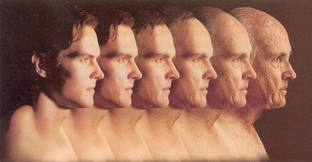
\includegraphics[width=0.95\linewidth]{images/viola/aging}
\-
                    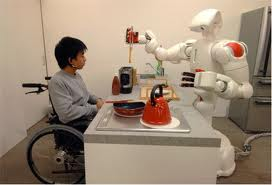
\includegraphics[width=0.95\linewidth]{images/viola/disabilities}
\-                                                                                  
		    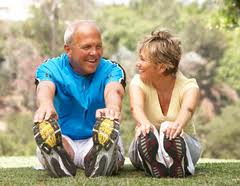
\includegraphics[width=0.95\linewidth]{images/viola/exercise}
\-

                \end{column}
              \end{columns}
            \end{block}

            \vfill
            
             \begin{block}{Cognitive Monitoring BCI application for Assitive Robotics}
               \begin{itemize}
              \item \textbf{Objectives}
                \begin{itemize}
                \item Develop a Cognitive Monitoring Non-invasive BCI mobile device.
                \item Real Time, Online, Single Trial, Active, Wearable, 
                \item It will assist both, subjects with limited but remanent walking abilities, and their therapists, by providing valuable feedback in rehabilitation procedures.
                \end{itemize}
              \end{itemize} 
              
		\centering
                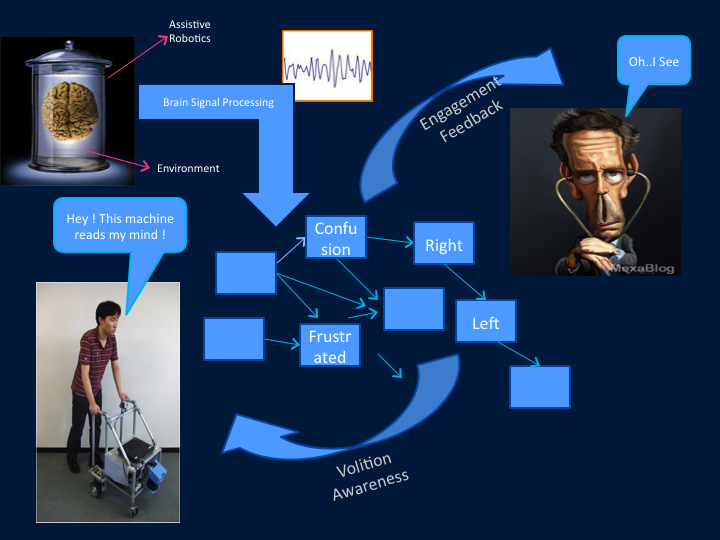
\includegraphics[width=0.90\linewidth]{images/viola/objective}

              \begin{itemize}
              \item \textbf{Research Questions: Work in progress }
                \begin{itemize}
                \item Does an Active BCI-powered assistive device allows better controllability and maneuverability?
                \item Is it possible to use Passive BCI (e.g. without user awareness) to enhance the safety of an assistive walking device ?
                \item Rehabilitation procedures are improved by using a Cognitive Monitoring BCI device ?  
                \item Is it possible to achieve an improved BCI device in terms of Cost, Throughput, Utility, Integration and Appearance ? [6]             
                \end{itemize}
              \end{itemize} 			  

            \end{block}
     
            \vfill

            \begin{block}{References and Previous Works}
              \begin{itemize}
                \item [1] \small Clark, Andy. Supersizing the Mind: Embodiment, Action, and Cognitive Extension: Embodiment, Action, and Cognitive Extension. Oxford University Press, 2008.
                \item [2] \small A. Cherubini, G. Oriolo, F. Macri, F. Aloise, F. Babiloni, F. Cincotti, and D. Mattia. Development of a
multimode navigation system for an assistive robotics project. \textit{Proceedings 2007 IEEE International
Conference on Robotics and Automation}, pages 2336–2342, April 2007.
                \item [3] Ionta, Silvio, Roger Gassert, and Olaf Blanke. Multi-sensory and sensorimotor foundation of bodily self-consciousness–an interdisciplinary approach. \textit{Frontiers in psychology 2 (2011)}.
                \item [4] Bahramisharif, Ali, et al. "Lateralized responses during covert attention are modulated by target eccentricity." \textit{Neuroscience letters} 491.1 (2011): 35-39.
                \item [5] Tan Desney S.  (Editor), Nijholt Anton (Editor)  et al, \textit{Brain-Computer Interfaces: Applying our minds to Human-Computer Interaction},2010, Springer
                \item [6] Allison, Brendan Z. "Toward ubiquitous bcis." Brain-Computer Interfaces. Springer Berlin Heidelberg, 2010. 357-387.
              \end{itemize}

            \end{block}
          }
          % ---------------------------------------------------------%
          % end the column
        \end{minipage}
      \end{beamercolorbox}
    \end{column}
    % ---------------------------------------------------------%
    % end the column
  \end{columns}
  \vskip1ex
  %\tiny\hfill\textcolor{ta2gray}{Created with \LaTeX \texttt{beamerposter}  \url{http://www-i6.informatik.rwth-aachen.de/~dreuw/latexbeamerposter.php}}
  % \tiny\hfill{Created with \LaTeX \texttt{beamerposter}  \url{http://www-i6.informatik.rwth-aachen.de/~dreuw/latexbeamerposter.php} \hskip1em}
\end{frame}
\end{document}


%%%%%%%%%%%%%%%%%%%%%%%%%%%%%%%%%%%%%%%%%%%%%%%%%%%%%%%%%%%%%%%%%%%%%%%%%%%%%%%%%%%%%%%%%%%%%%%%%%%%
%%% Local Variables: 
%%% mode: latex
%%% TeX-PDF-mode: t
%%% End:
